\documentclass[11pt]{exam}
%\usepackage{euscript}

\usepackage{amsmath}
\usepackage{amsthm}
\usepackage{amssymb}
\usepackage{epsfig}
\usepackage{xspace}
\usepackage{color}
\usepackage{url}
\usepackage{subfig}
\usepackage{float}
\usepackage{array}
\graphicspath{ {images/} }
%%%%%%%  For drawing trees  %%%%%%%%%
\usepackage{tikz}
\usetikzlibrary{calc, shapes, backgrounds}

%%%%%%%%%%%%%%%%%%%%%%%%%%%%%%%%%
\setlength{\textheight}{9in}
\setlength{\topmargin}{-0.600in}
\setlength{\headheight}{0.2in}
\setlength{\headsep}{0.250in}
\setlength{\footskip}{0.5in}
\flushbottom
\setlength{\textwidth}{6.5in}
\setlength{\oddsidemargin}{0in}
\setlength{\evensidemargin}{0in}
\setlength{\columnsep}{2pc}
\setlength{\parindent}{1em}
%%%%%%%%%%%%%%%%%%%%%%%%%%%%%%%%%


\newcommand{\eps}{\varepsilon}

\renewcommand{\c}[1]{\ensuremath{\EuScript{#1}}}
\renewcommand{\b}[1]{\ensuremath{\mathbb{#1}}}
\newcommand{\s}[1]{\textsf{#1}}
\newcommand{\tb}[1]{\textbf{#1}}

\newcommand{\E}{\textbf{\textsf{E}}}
\renewcommand{\Pr}{\textbf{\textsf{Pr}}}
%\footnote{\s{CS 6140  Data Mining; \;\; Spring 2015 \hfill
%Instructor: Jeff M. Phillips, University of Utah}
%}

\title{CS 6140 Data Mining Project Intermediate Report}
\author{Padmashree Teeka (u0880562), Roshani Nagmote (u0941394), Anirudh Narasimhamurthy (u0941400)}

\begin{document}

\maketitle

\textbf{\underline{•} Comparing performances of different Clustering Techniques on the dataset.}

%\begin{center}
%	\textbf{\underline{C}
%\end{center}
%
%

\section{What progress you have made towards your proposed goal?}

\begin{itemize}
	
 \item[] Our proposed goal was to perform different clustering techniques on social network dataset. We chose LiveJournal dataset as our input data set to work on. We plan on performing 3 clustering techniques on our dataset. They are: 
\begin{enumerate}
	
\item  Hierarchical Clustering
\item  Spectral Clustering
\item  K-means Clustering 

\end{enumerate}

\item \textbf{Hierarchical Clustering}
\begin{itemize}
\item  Analysing and finalizing on the distance measure to be used for the graph datasets for performing hierarchical clustering.
\item Coming up with basic clustering algorithm which works on relatively smaller graph
\item Looking at options for scaling our algorithm to work on larger data and overcoming memory issues.
\end{itemize}

\item \textbf{Spectral Clustering}

\begin{itemize}

\item Constructing the basic adjacency matrices, degree matrices and the normalized Laplacian required for performing spectral clustering.
\item Identifying the need to construct sparse adjacency matrices to avoid memory issues when the graph data contains nodes in the order of 1 million nodes.
\item Coming up with an algorithm which performs spectral clustering by identifying where the cuts have to be made on the edges in the graph.

\end{itemize}	

\item \textbf{K-means Clustering}
\begin{itemize}
\item  Understanding and working on the algorithm.
\item Working on how to provide centers for our k-means algorithm.
\end{itemize}


\end{itemize}

\section{ If you tried some basic approaches: what worked well and what did not }

\begin{itemize}
%Our dataset basically has from nodes and to nodes and we are supposed to find communities in this dataset. So, we referred this paper which discusses about community detection problems with different clustering techniques.  \\
%
%http://snap.stanford.edu/class/cs224w-readings/fortunato10community.pdf

\item\textbf{Hierarchical Clustering}

The basic approaches which worked are as follows:
\begin{itemize}
	\item Deciding to use Hamming distance as the distance measure for performing bottom-up clustering on graph datasets worked for smaller toy graph datasets.

	\item The distance measure used in our code was : \\
	$d^{HAD}(i,j)=\sum_{k=0}^{n-1}[y_{i,k} \neq y_{j,k}]$ 

where, $d^{HAD}$ is the Hamming distance between rows of our Adjacency Matrix.

Hamming distance was found by finding difference between each of the row elements of our adjacency matrix by finding the percentage of the nodes that differ. 

\item Having the distance vector reformed into a Square matrix made the computation easier. 
\end{itemize}
 
The basic approaches which did not work are as follows:
\begin{itemize}
	\item Computing the Hamming distance between clusters when the number of nodes is in the order of 1 million nodes failed with an out of memory error in MATLAB as storing and processing them becomes difficult.
	\item We were able to explore other option of using sparse adjacency matrix but will have to check if computing Hamming distances using the sparse matrices would give us the correct distances required for hierarchical clustering.

\end{itemize}

\item\textbf{Spectral Clustering}\\

The basic approaches which worked are as follows:
\begin{itemize}
	\item Constructing a full adjacency matrix for the given undirected graph of smaller size.
	\item Constructing a normalized/ unnormalized Laplacian for the dataset.
	\item For the given problem, we found the Fiedler vector, which is eigen vector corresponding to the second smallest eigenvalue of the Laplacian matrix to be a very good descriptor for the graph. We were able to implement and get the correct Fiedler vector for the smaller dataset, which gave us an idea as to where the cuts were to be made for the spectral clustering.
	\item We ran the spectral clustering on  a graph which contains 1049866 nodes and we were able to obtain \emph{k-partitioned group of nodes} based on the input value of k. A plot of the adjacency matrix is shown below:
\end{itemize}

The basic approaches which did not work are as follows:
\begin{itemize}
	\item Constructing an adjacency matrix directly from the given information about To and From nodes did not create the square/ symmetric adjacency matrix which we required.
	\item Working with a full adjacency matrix for spectral clustering also doesn't work when the number of nodes in the graph is in the order of millions. We overcame this by using sparse adjacency matrices.
	\item The clustering we get when we run on a dataset with 1 million nodes is shown in \textbf{Appendix} 
	

	
\end{itemize}

\item\textbf{K-means Clustering}
\begin{itemize}

\item We are working on initializing centers for K-means algorithm using k-means++ algorithm. Once this is done we hope to zero in on the distance measure for labelling the nodes into the newly formed cluster. 

\end{itemize}

\end{itemize}

\section{What could be done to improve the basic approaches?}

\begin{itemize}

\item \textbf{ Hierarchical Clustering}:

\begin{itemize}
	\item  Since our algorithm was running into memory constraints while trying to compute the Hamming distances for the graph datset will 1 million nodes, one possible approach could be to split the data into smaller chunks and then perform the computation on the smaller chunk.
\end{itemize}	
\item \textbf{ Spectral Clustering}:
\begin{itemize}
	\item Similar memory constraints issues were faced when we were trying to run our basic spectral clustering algorithm on our huge dataset. One of the possible solutions which we came across was to make use of a datastore which would allow us to process data which are too large to fit in memory.
	\item We also found that when we ran our algorithm for a million nodes on the CADE machines which have memory of 16GB, we were able to process, but we couldn't run it on our local machines.
	\item We are still exploring options for visualizing the clusters formed from spectral clustering.
\end{itemize}

\item \textbf{ K-means Clustering}:
\begin{itemize}

\item Once we have our basic approach working, we can probably run the algorithm multiple times till it converges to a local minimum. We also plan to improve the initialization of centroids. Also, we would like to explore how many clusters are appropriate for a k-means clustering algorithm.

\end{itemize}

\end{itemize}
\section{What experiments have you run and are you planning to run to demonstrate the effectiveness}

\begin{itemize}

\item We adopted the approach of testing out our algorithm on relatively small, medium and large datasets. We found our spectral and hierarchical clustering algorithms work well for very small datasets which was expected.

\item When we ran it across a graph with 1 million nodes, our spectral clustering algorithm was able to produce the clusters while our hierarchical clustering failed due to memory issues. We are working on this issue.

\item Once we have the correct approach to load/ store /process large graphs, we are planning to run it on large graph datasets of social networks and would be interested to see the results it is providing us.
\end{itemize}


\section{Appendix}

\begin{itemize}
	\item We are exploring ways to visualize our clusters.We have got our edges where the cut needs to be made. We did do a sanity check and tried visualizing the sparse matrix which we created using spy function in MATLAB and the output is shown below:
\end{itemize}

\begin{center}
	
	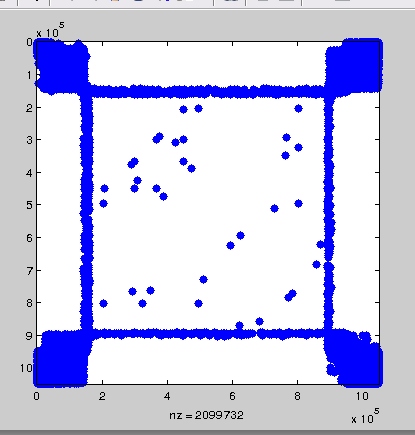
\includegraphics[width=.7\linewidth]{spec10.png}
	
	%keep a line empty after include graphics 
	
\end{center}

\end{document}
